\section{设计模式的引入}

\subsection{引入设计模式的作用}

\subsubsection{共享词汇}
下图以餐厅点单为例。服务员和厨师之间有“共享的词汇”,顾客却不懂这生词汇。共享的词汇不仅方便顾客点餐,也让厨师不用记太多事,毕竞这些餐点模式都已经在他的脑海中了。

同样的,设计模式让你和其他开发人员之间有共享的词汇,一旦懂得这些词汇,和其他开发人员之间沟通就很容易,也会促使那些不懂的程序员想开始学习设计模式。设计模式也可以把你的思考架构的层次提高到模式层面,而不是仅停留在琐碎的对象上。

\begin{figure}[H]
    \vspace{-0.5em}
	\centering
	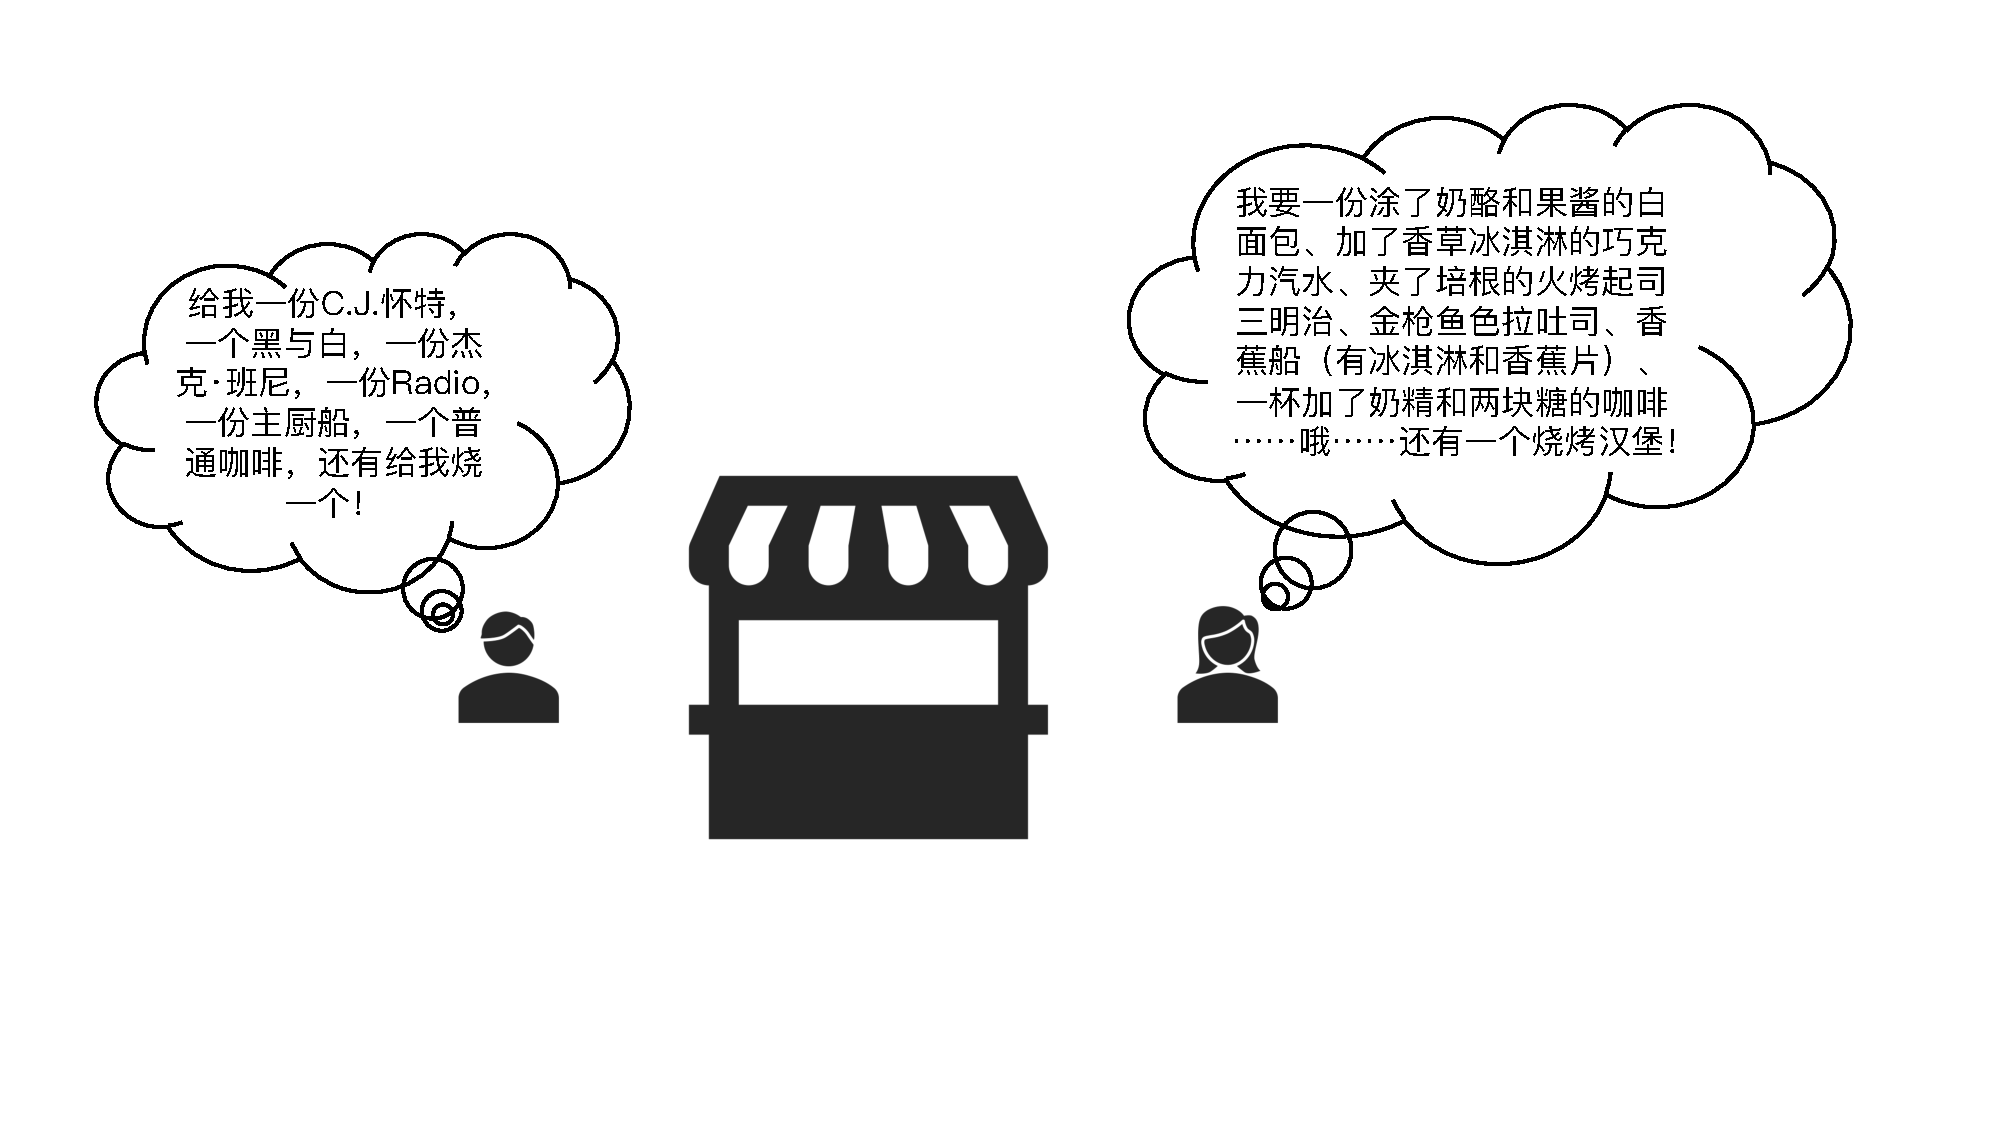
\includegraphics[width=0.8\textwidth]{images/共享词汇.pdf}
    \vspace{-1em}
\end{figure}

\subsubsection{共享模式词汇的力量}
\begin{itemize}
    \item \textbf{共享的模式词汇“威力强大”。}当你使用模式名称和其他开发人员或者开发团队沟通时,你们之间交流的不只是模式名称,而是一整套模式背后所象征的质量、特性、约束。
    \item \textbf{模式能够让你用更少的词汇做更充分的沟通。}当你用模式描述的时候,其他开发人员便很容易地知道你对设计的想法。
    \item \textbf{将说话的方式保持在模式层次,可让你待在“设计圈子”久一点。}使用模式谈论软件系统,可以让你保持在设计层次,不会被压低到对象与类这种琐碎的事情上面。
    \item \textbf{共享词汇可帮你的开发团队快速充电。}对于设计模式有深入了解的团队,彼此之间对于设计的看法不容易产生误解。
    \item \textbf{共享词汇能帮助初級开发人员迅速成长。}初级开发人员向有经验的开发人员看齐。当高级开发人员使用设计模式,初级开发人员也会跟着学。把你的组织建立成一个模式使用者的社区。
\end{itemize}

\subsection{库与设计模式}
\begin{figure}[H]
    \vspace{-0.5em}
	\centering
	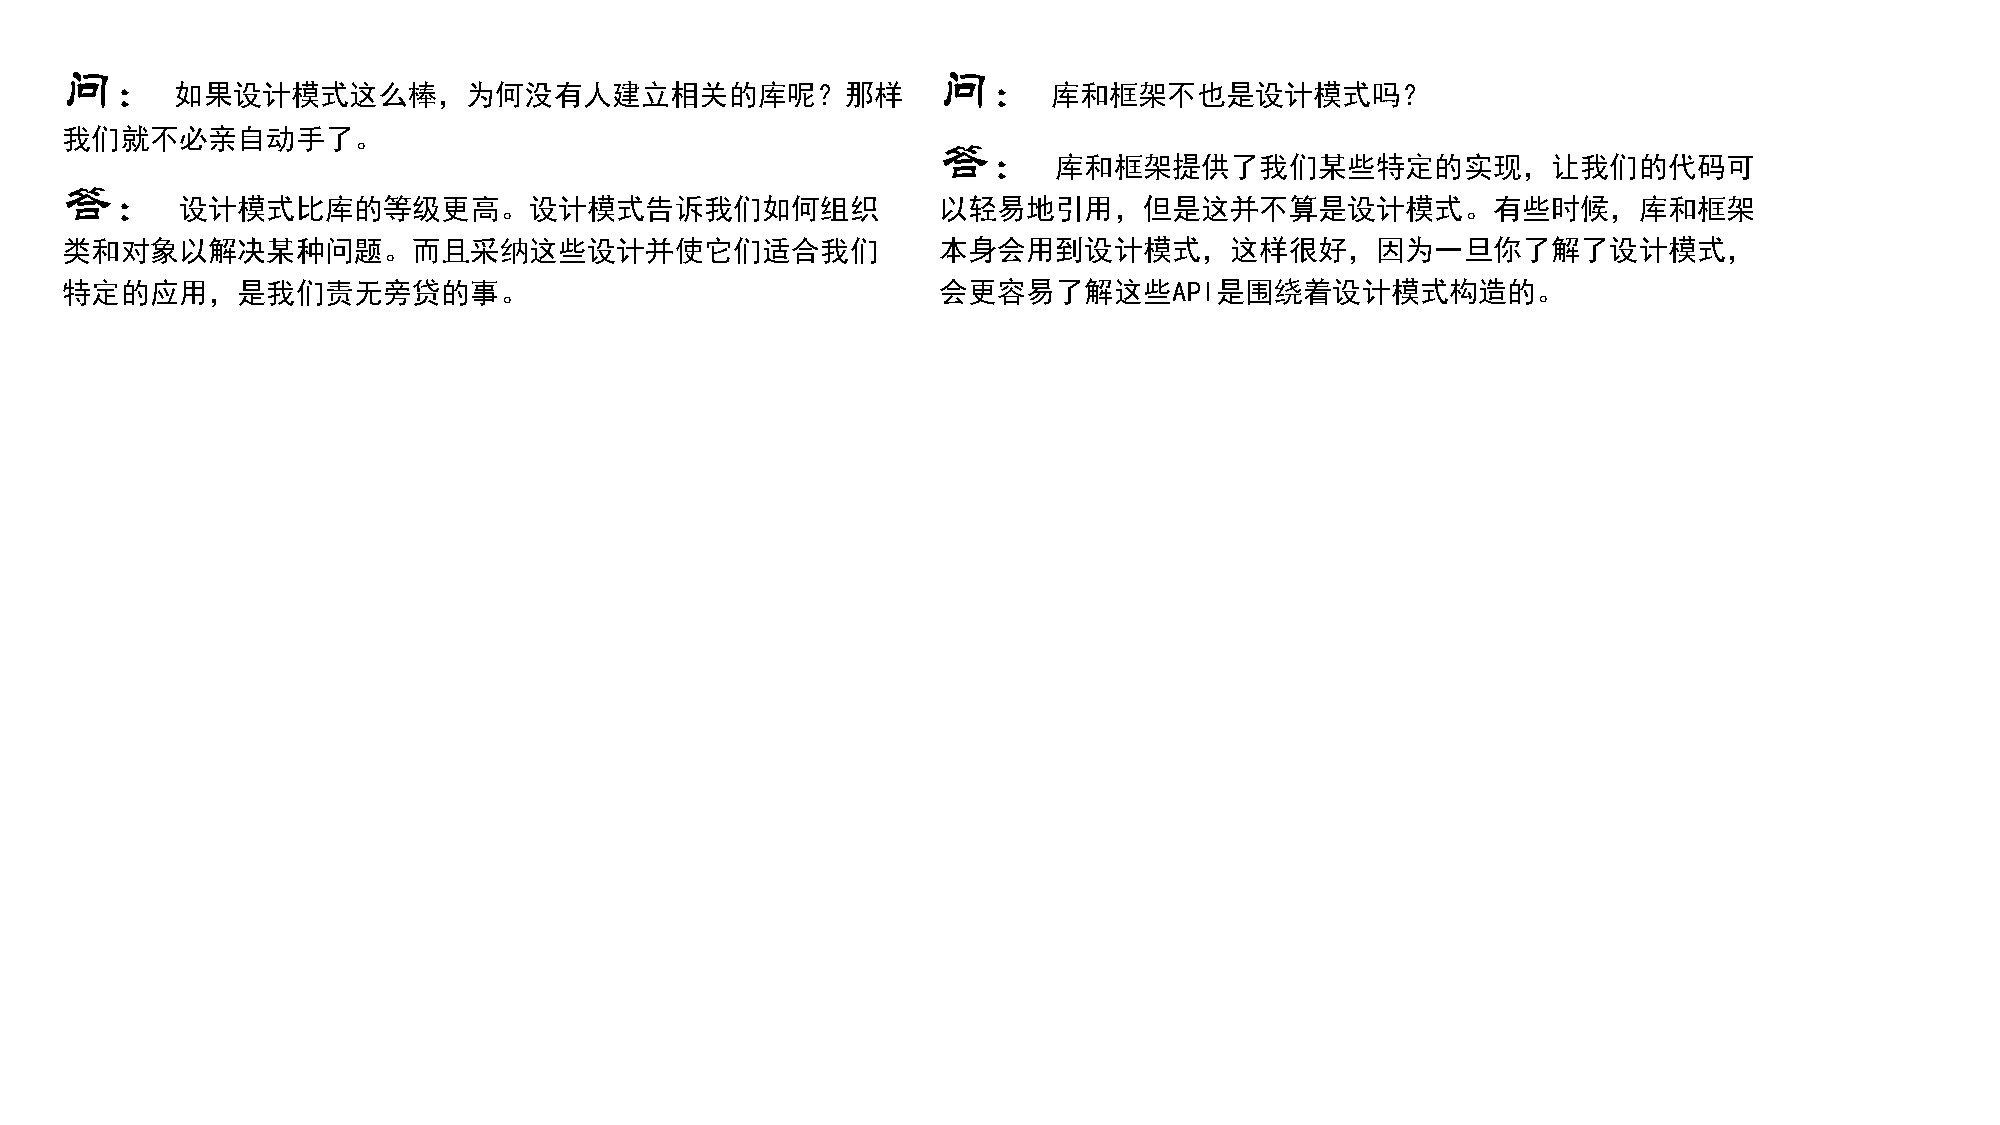
\includegraphics[width=\textwidth]{images/库与设计模式.pdf}
    \vspace{-1em}
\end{figure}

\subsection{要点总结}
\begin{itemize}
    \item 知道OO基础,井不足以让你设计出良好的OO系统。
    \item 良好的OO设计必须具备可复用、可扩充、可维护三个特性。
    \item 模式可以让我们建造出具有良好OO设计质量的系统。
    \item 模式被认为是历经验证的OO设计经验。
    \item 模式不是代码,而是针对设计问题的通用解决方案。你可把它们应用到特定的应用中。
    \item 模式不是被发明,而是被发现。
    \item 大多数的模式和原则,都着眼于软件变化的主题。
    \item 大多数的模式都允许系统局部改变独立于其他部分。
    \item 我们常把系统中会变化的部分抽出来封装。
    \item 模式让开发人员之间有共享的语言,能够最大化沟通的价值。
\end{itemize}




